% !TEX TS-program = XeLaTeX

% STYLE

\documentclass[a4paper, 12pt]{article}
\usepackage[left=1in,
		    right=1in,
    		    top=1in,
		    bottom=1in,
		    bindingoffset=0cm]{geometry}
		    \usepackage{array}
\usepackage{float}
\usepackage{graphicx}
\graphicspath{ {./images/} }
\usepackage{subfig}
\usepackage{enumerate}
\usepackage[normalem]{ulem} % underlining
\usepackage{booktabs} % tables
\usepackage[table]{xcolor} % coloring tables
\newcolumntype{L}[1]{>{\raggedright\let\newline\\\arraybackslash\hspace{0pt}}m{#1}} % beautiful column types
\newcolumntype{C}[1]{>{\centering\let\newline\\\arraybackslash\hspace{0pt}}m{#1}}

% LANGUAGE + FONT
		    
\usepackage[english]{babel}
\usepackage[backend=biber,
                     style=unified]{biblatex}
\newcommand{\citeay}[2][]{\citeauthor{#2} (\citeyear[#1]{#2})}
\addbibresource{ref.bib}
\usepackage{fontspec}  
\setmainfont{Minion 3}
\usepackage{pifont}
\usepackage{bbding}

% DRAWING

\usepackage{tikz}
\usepackage{tikz-qtree}
\usetikzlibrary{shapes.geometric}
\usetikzlibrary{trees,arrows}
\usetikzlibrary{positioning}
\usetikzlibrary{matrix}
\usetikzlibrary{tikzmark}
\usetikzlibrary{decorations.shapes}
\usetikzlibrary{decorations.pathmorphing}

% LINGUISTICS 

\usepackage{expex}
\usepackage[glossaries]{leipzig}
\makeglossaries
\newleipzig {npst} {npst} {non-past}
\newleipzig {nfin} {nfin} {non-finite}
\newleipzig {nsg} {nsg} {non-singular}
\newleipzig {part} {part} {partitive case}
\newleipzig {pot} {pot} {potentialis}

\lingset{numoffset=1ex, aboveexskip=1em, belowexskip=1em}

\title{Consonant gradation}
\author{Sasha Shikunova, EGG2023, Novi Sad}
\date{Last updated \today}

\begin{document}
\maketitle

	\section{Definitions}
	
	\ex Consonant gradation, also known as ``grade alternation'', is a subtype of consonant mutation occurring in the inflection and derivation of all parts of speech. It is a systematic morphophonological alternation of consonants on the border of two syllables, resulting in either weakening or strengthening of consonants. \trailingcitation{\parencite[p. 859]{bakronagy2022}}
	\xe
	Some consonant grade alternation examples from Estonian \parencite{trosterud-uibo2005}.
	
	\begin{enumerate}[$\gg$]
		\item nouns: 
			\begin{enumerate}[$\cdot$]
				\item {\Sg} {\Nom} ({\Sg} {\Part}) -- strong grade
				\item {\Sg} {\Gen} -- weak grade
			\end{enumerate}
		\item verbs: 
			\begin{enumerate}[$\cdot$]
				\item supine (primary form) -- strong grade
				\item indicative mode present tense -- weak grade 
			\end{enumerate} 
	\end{enumerate}
	
	\begin{figure}[H]
		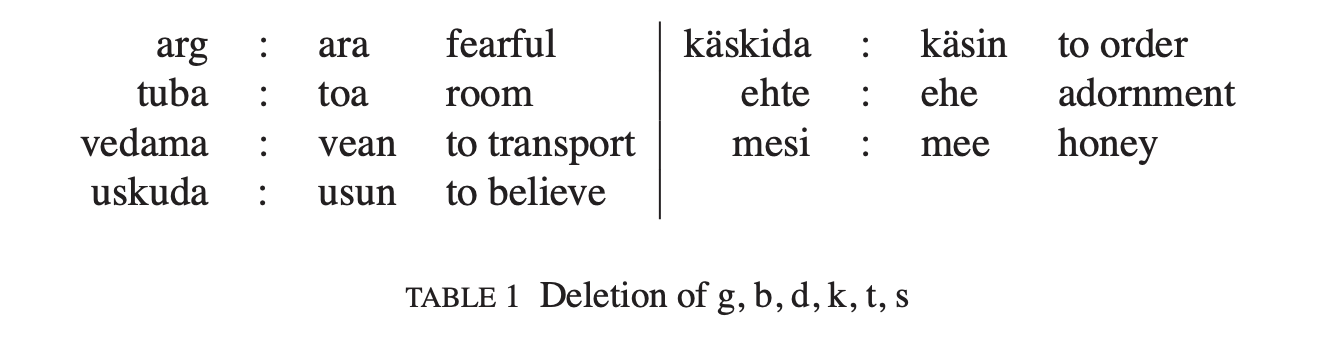
\includegraphics[scale=.6]{est-grades1}
	\end{figure}
	
	\begin{figure}[H]
		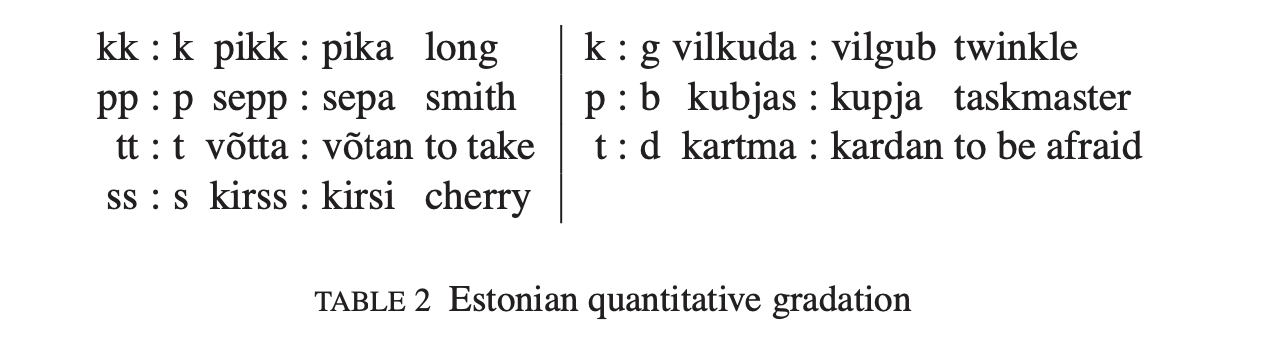
\includegraphics[scale=.6]{est-grades2}
	\end{figure}
	\parencite[pp. 139--140]{trosterud-uibo2005}
	
	\begin{enumerate}[$\gg$]
		\item Consonant grade alternations are prominent in Finnic languages: Finnish, Estonian, Saami, Karelian, etc.
		\item In the Estonian examples above, sometimes the change is positional: intervocalically, consonants undergo lenition (\emph{pikk} : \emph{pika})
		\item Sometimes, however, the alternation happens despite the consonants being in similar positions: \emph{v{\~o}tta} : \emph{v{\~o}tan}
		\\$\Rightarrow$ consonant gradation can be morphologised 
	\end{enumerate}
	What is so special about consonant gradation?
	
	\begin{enumerate}[$\gg$]
		\item It is not fully phonologically motivated on the synchronic level but sometimes productive (Nganasan)
		\item How did it develop? Sometimes triggers of grade alternations disappear but the alternations themselves remain
		\item Three-way distinctions may be a problem for autosegmental CVCV representations
	\end{enumerate}
	So, what types of consonant gradation exist and how are they described?
	
			\subsection{Realisation of consonant grades}
			
	Grades can be realised via quality or quantity. Qualitative alternations include: 
%	weakening can mean shortening (degemination) or cluster simplifica- tion; the qualitative forms of weakening include voicing, fricativization, approximation and loss of consonants, as well as assimilation in consonant clusters, resulting in geminate consonants
	
	\begin{enumerate}[$\gg$]
	\setlength\itemsep{0em}
		\item voicing : /k/ $\leftrightarrow$ /g/
		
		\ex Finnish\\
			\emph{alanko} -- \emph{alango-n} \hfill `lowland.{\Nom}' -- `lowland.{\Gen}'
		\xe
		
		\item fricativisation : /t/ $\leftrightarrow$ /ð/
				
		\pex Inari Saami \parencite{valtonen2022}
			\a \emph{neeti} /neːti/ -- \emph{neđe} /neðe/ \hfill `marten.{\Nom}' -- `marten.{\Gen}'
			\a \emph{tupe} /tupe/ -- \emph{tuve} /tuve/ \hfill `cabin.{\Nom}' -- `cabin.{\Gen}'
		\xe
		
		\item assimilation (cluster simplification) : /nd/ $\leftrightarrow$ /nn/
		
		\ex Karelian \parencite{ryagoev1993}\\
			\emph{kandua} -- \emph{kannan} \hfill `to carry' -- `I carry'
		\xe
		
		\item approximation : /g/ $\leftrightarrow$ /v/
		
		\ex Karelian \parencite{ryagoev1993}\\
			\emph{ruga} -- \emph{ruvan} \hfill `soft resin.{\Nom}' -- `soft resin.{\Gen}'
		\xe
		
	\end{enumerate}
	
	\noindent Quantitative alternations:
%	As a quantitative alternation, weakening can mean shortening (degemination) or cluster simplifica- tion + deletion
	
	\begin{enumerate}[$\gg$]
	\setlength\itemsep{0em}
		\item (de)gemination : /kk/ $\leftrightarrow$ /k/
		
		\ex Finnish\\
			\emph{pappi -- papit} \hfill `priest.{\Nom}' -- `priest.{\Pl}'
		\xe
		
		\item alternation between long and super-long geminates : /ppp/ $\leftrightarrow$ /pp/
		
		\ex Estonian\\
			\emph{pikk} /pikkk/ -- \emph{pika} /pikka/ \hfill `long.{\Nom}' -- `long.{\Gen}'
		\xe
		
		\item loss : /b/ $\leftrightarrow$ ø
		
		\ex Estonian\\
			\emph{tuba -- toa} \hfill `room.{\Nom}' -- `room.{\Gen}'
		\xe
	Within one paradigm, the set of alternating consonant grades is usually of size 2 but can be larger: Skolt Saami can have 3 or 4 grades alternating within the paradigm of one word \parencite{koponen2022}. This is a problem for Strict CV representations
	
	\begin{enumerate}[$\cdot$]
	\setlength\itemsep{0em}
		\item Strong grade: long geminate
		\item Weak grade: short geminate
		\item Shortened grade: single consonant
	\end{enumerate}
	
	\begin{figure}[H]
		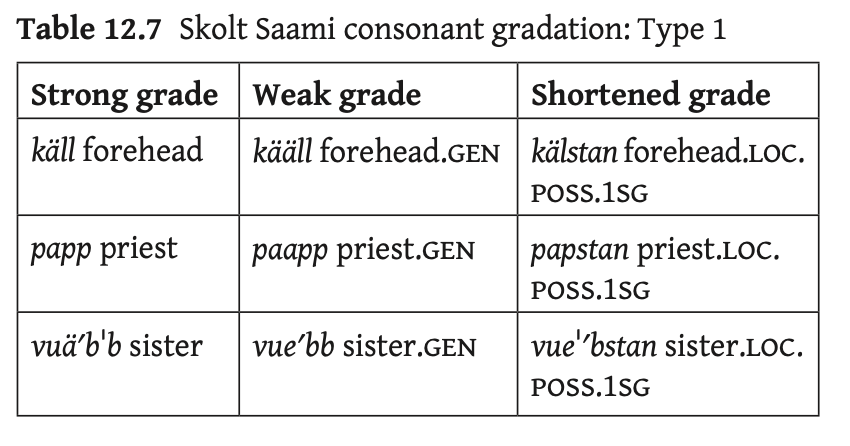
\includegraphics[scale=.6]{skolt-grades1}
	\end{figure}
	
	\begin{enumerate}[$\cdot$]
	\setlength\itemsep{0em}
		\item Lengthened grade: long geminate
		\item Strong grade: short geminate
		\item Weak grade: single consonant
		\item Shortened grade: single consonant
	\end{enumerate}
	
	\begin{figure}[H]
		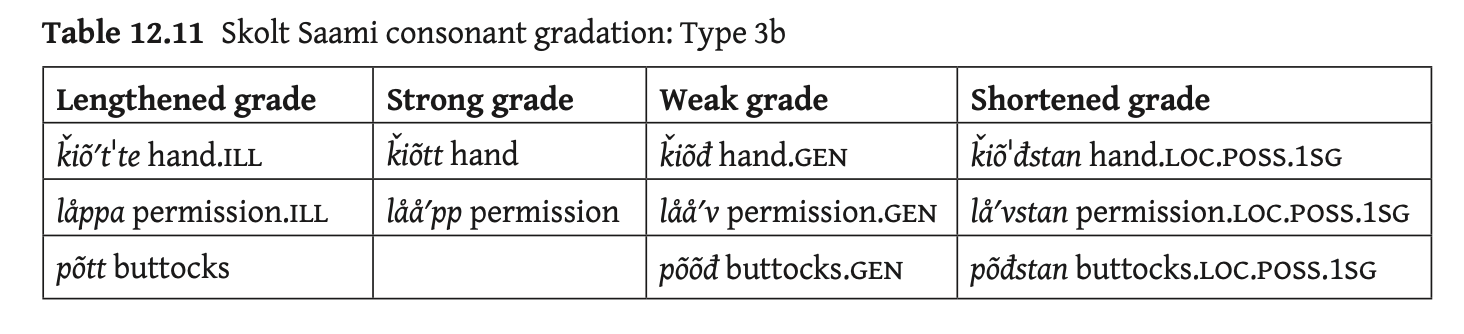
\includegraphics[scale=.6]{skolt-grades2}
	\end{figure}
		
	\end{enumerate}
	Grade alternations have triggers, targets and domains:
	
	\begin{enumerate}[$\gg$]
	\setlength\itemsep{0em}
		\item \textsc{Trigger} -- a phonological entity that causes the alternation (e.g. suffix)
		\item \textsc{Target} -- the consonant whose grade is affected
		\item \textsc{Domain} -- the phonological unit within which the alternation happens; the smallest relevant unit
	\end{enumerate}
	The trigger and target of a consonant grade alternation do not have to be directly adjacent. Wrt. triggers, target and domains, these alternations are divided into two types:
	
	\begin{enumerate}[$\gg$]
		\item \textsc{Radical (syllabic) gradation} -- occurs in the root, between the first (stressed) and the second (unstressed) syllable
		
		\pex Finnish radical gradation (quantitative; semi-productive)
			\a \emph{pappi} `priest' : \emph{papit} `priests'
			\a \emph{lobbaan} : \emph{lobata} `to lobby'
		\xe
		
		\pex~ Estonian radical gradation
			\a \emph{arg} : \emph{ara} `fearful'
			\a \emph{sepp} : \emph{sepa} `smith' \trailingcitation{\parencite[pp. 139--140]{trosterud-uibo2005}}
		\xe
		
		\item \textsc{Suffixal (rhythmic) gradation} -- usually applies to suffix-initial consonants, conditioned by syllable count (odd stressed vs even unstressed)
		
		\pex North Saami suffixes \parencite[p. 149]{korhonen1981}
			\a \emph{læǯǯap} `be.{\Pot}.{\Fpl}'
			\a \emph{m\^{a}n\^{a}ǯæp} `go.{\Pot}.{\Fpl}'
		\xe
		
		\pex~ Forest Nenets durative \parencite[p. 359]{salminen2007}
			\a \emph{kata-pʹo-} `kill-{\Dur}'
			\a \emph{ta-mʹpʹo-} `bring-{\Dur}'
		\xe
		\item What is the difference if both take into account foot structure and stress?
	\end{enumerate}
	The trigger of syllabic gradation is often a consonant closing the syllable \emph{after} the target of gradation (\ref{fingrad}). So, the trigger and the target are not adjacent because they are separated by a nucleus.  
		
	In Finnish, the gradation process has extended to occur after all syllables -- stressed and unstressed. 
	
	\pex\label{fingrad}Finnish syllabic gradation
		\a \emph{sukka} `sock' : {\Gen} \emph{suka-n}
		\a \emph{alanko} `lowland': {\Gen} \emph{alango-n} \trailingcitation{\parencite[p. 862]{bakronagy2022}}
	\xe
	So, syllabic gradation extended to all syllables is no longer rhythmically motivated; its trigger is still working.

	\section{Estonian puzzle}
	
	Consonant and vowel inventories \parencite{asu-teras2009}
	
	\begin{figure}[H]
		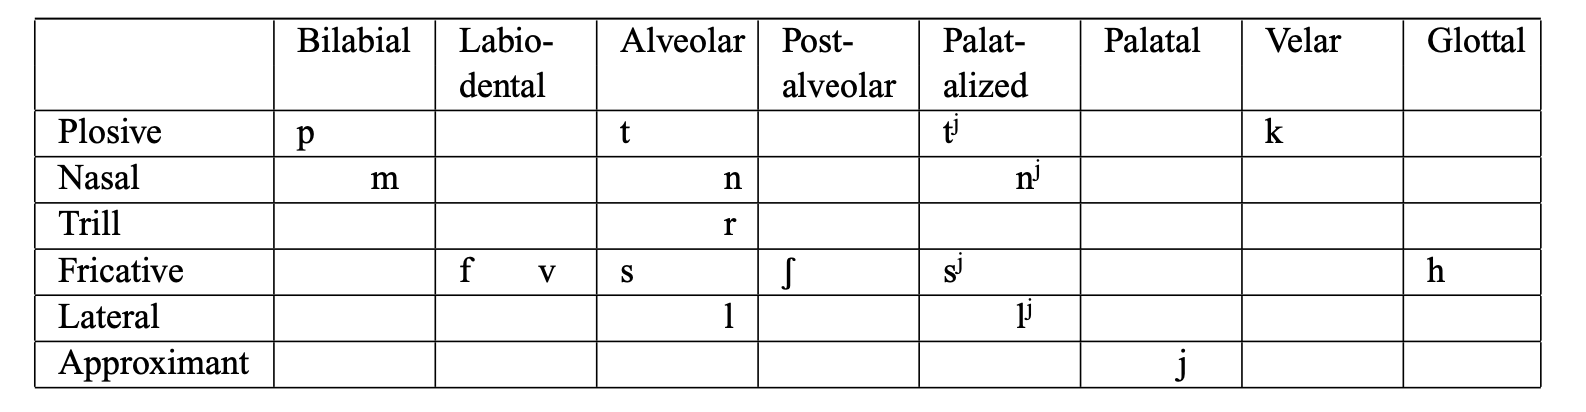
\includegraphics[scale=.6]{est-consonants}
	\end{figure}
		
	\begin{figure}[H]
		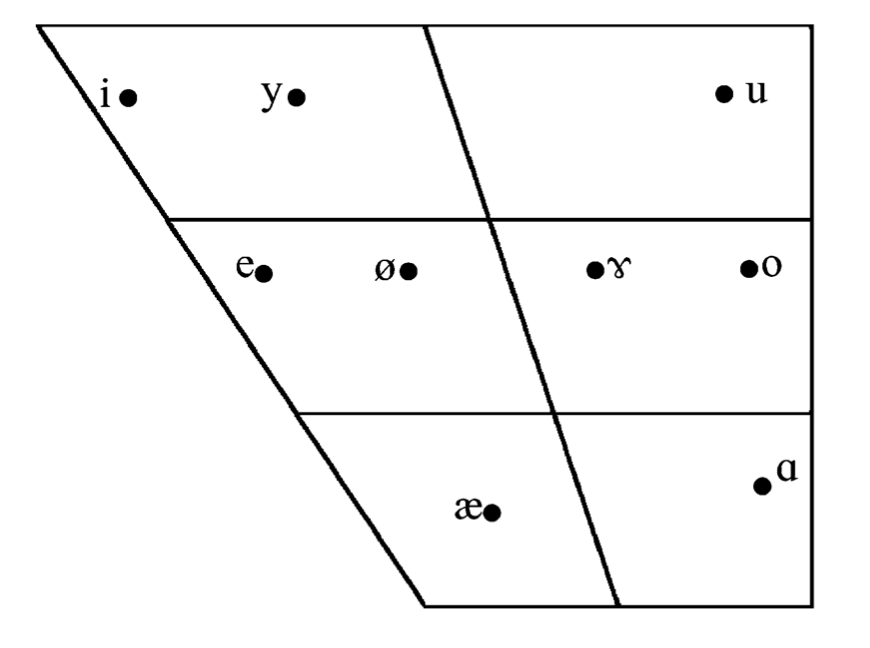
\includegraphics[scale=.5]{est-vowels}
	\end{figure}

	\section{Consonant gradation data}
	
	Several verbs in 5 different forms \parencite{problems}.

\begin{table}[H]
\begin{tabular}{llllll}
\toprule
\textbf{Infinitive I} & \textbf{Infinitive II} & \textbf{Present tense} & \textbf{Past tense} & \textbf{Participle} & \textbf{Translation} \\
\midrule
hakkama               & hakata                 & hakkan                 & hakkasin            & hakatud             & begin                \\
\addlinespace[0.2cm]
hüppama               & hüpata                 & hüppan                 & hüppasin            & hüpatud             & jump                 \\
\addlinespace[0.2cm]
näitama               & näidata                & näitan                 & näitasin            & näidatud            & show                 \\
\addlinespace[0.2cm]
kompima               & kompida                & kombin                 & kompisin            & kombitud            & feel, touch          \\
\addlinespace[0.2cm]
lõikama               & lõigata                & lõikan                 & lõikasin            & lõigatud            & cut                  \\
\addlinespace[0.2cm]
õppima                & õppida                 & õpin                   & õppisin             & õpitud              & study, learn         \\
\addlinespace[0.2cm]
põdema                & põdeda                 & põen                   & põdesin             & põetud              & be sick              \\
\addlinespace[0.2cm]
pumpama               & pumbata                & pumpan                 & pumpasin            & pumbatud            & pump                 \\
\addlinespace[0.2cm]
sulgema               & sulgeda                & sulen                  & sulgesin            & suletud             & close                \\
\addlinespace[0.2cm]
rääkima               & rääkida                & räägin                 & rääkisin            & räägitud            & speak                \\
\addlinespace[0.2cm]
tõlkima               & tõlkida                & tõlgin                 & tõlkisin            & tõlgitud            & translate           \\
\bottomrule
\end{tabular}
\end{table}

	\begin{enumerate}[$\cdot$]
		\item g $\rightarrow$ /k/
		\item k $\rightarrow$ /kk/
		\item kk $\rightarrow$ /kkk/
	\end{enumerate}

		\subsection{Questions and answers}
	
\begin{enumerate}[$\gg$]
	\item How many consonant grades does Estonian have?\\
	There are 4 grades:
\begin{table}[H]
\begin{tabular}{cccc}
1  & 2 & 3 & 4 \\
pp & p & b & ø \\
tt & t & d & ø \\
kk & k & g & ø
\end{tabular}
\end{table}
	\item Which of the forms is the most ``basic'' one, from which all the other are produced? \\
		The basic form should be Infinitive II -- other forms are produced from it. In Infinitive II, the ending \emph{ta/da} tells us whether the present tense should have a weak or a strong grade.
		\begin{enumerate}[$\cdot$]
			\item \emph{-da} $\Rightarrow$ weak grade in the present tense
			\item \emph{-ta} $\Rightarrow$ strong grade in the present tense
		\end{enumerate}
	\item What are the rules that produce each form?\\
	Take Infinitive II, strip the ending (\emph{da/ta}), then apply the gradation rule to the base. Strong grade is the same as in Infinitive II, weak grade is one grade weaker.\\
	
	\begin{minipage}{.45\textwidth}
	For the \emph{da} class:
		\begin{enumerate}[$\cdot$]
		\setlength\itemsep{0em}
			\item Infinitive I -- strong grade + \emph{ma}
			\item Present tense -- weak grade + \emph{n}
			\item Past tense -- strong grade + \emph{sin}
			\item Participle -- weak grade + \emph{tud}
		\end{enumerate}
	\end{minipage}
	\hfill
	\begin{minipage}{.45\textwidth}
	For the \emph{ta} class:
		\begin{enumerate}[$\cdot$]
		\setlength\itemsep{0em}
			\item Infinitive I -- strong grade + \emph{ama/ima}
			\item Present tense -- strong grade + \emph{n}
			\item Past tense -- strong grade + \emph{sin}
			\item Participle -- weak grade + \emph{tud}
		\end{enumerate}
	\end{minipage}
\end{enumerate}
	
		\section{Grades in Substance-Free Phonology}
		
	There has been proposed phonetic motivation for radical gradation.
	
	\pex Radical gradation has always been caused by the need for greater articulatory energy in the closed syllable after the syllable with the main stress than in the open syllable. This brought about a corresponding drop in intensity at the preceding syllable juncture and a weakening of the [onset] consonant. \trailingcitation{\parencite[p. 275]{korhonen1988}}
	\xe
	However:
		
	\begin{enumerate}[$\gg$]
		\item The alternations are not always synchronically linked to the strength of the position (Finnish)
		\item In some cases, the strong grade of some segments actually takes less energy to produce (Guovdajohtolat Northern Saami)
	\end{enumerate}
	In the Guovdajohtolat dialect of Northern Saami, there are weak and strong consonant grades (\ref{norsaami}). /pp tt kk/ in the strong grade correspond to their voiced counterparts /bb dd gg/. What we observe in other languages with consonant gradation is voiced consonants occuring in weaker positions, which is more expected from the point of view of articulation: voiced stops are more difficult to hold than the unvoiced ones.
	
	\ex\label{norsaami}Northern Saami consonant gradation \parencite[p. 19]{balsbaal2007}\\
\begin{tabular}{cc}
strong grade & weak grade \\
...hp...           & ...p...          \\
...ʔm...           & ...m...          \\
...ss...           & ...s...          \\
...bb...           & ...pp...        
\end{tabular}
	\xe
	As noted by \citeay[p. 141]{chabot2021}, ``there is no phonetic explanation for how phonological lengthening could produce voicing of voiceless geminates'', which is an argument for the Substance-Free phonology view that phonological rules do not have to be phonetically grounded \parencite{hale-reiss2008}.
	
			\subsection{Russian iotation}
			
	A sharp pivot to Russian palatalisation and iotation, which Daniar Kasenov and I have proposed a grade-like treatment for \parencite{shikunova-kasenov2023}. The idea is parallel to 
	
	In Russian, there is a small class of suffixes which produce \emph{iotation}, one of them is the {\Fsg} ending \emph{-Ju}. Iotation is productive and affects recent loanwords.
	
\begin{minipage}[t]{0.45\linewidth}
	\ex\label{ex:exes}po\textbf{bud}ka -- \textbf{buž}u\hfill(d/ž alternation)\\
		\textbf{kos}a -- \textbf{koš}u\hfill (s/š alternation)\\
		u\textbf{klon}  -- \textbf{klon\textsuperscript{j}}u\hfill(n/n\textsuperscript{j} alternation)
	\xe
\end{minipage}
\hfill
\begin{minipage}[t]{0.45\linewidth}
	\ex\label{ex:exes-end}\textbf{l\textsuperscript{j}ub}ov\textsuperscript{j} -- \textbf{lyubl\textsuperscript{j}}u\hfill(b/bl\textsuperscript{j}  alternation)\\
		\textbf{sp}at\textsuperscript{j}  -- \textbf{spl\textsuperscript{j}}u\hfill(p/pl\textsuperscript{j}  alternation)\\
		\textbf{stav}ka  -- \textbf{stavl\textsuperscript{j}}u\hfill(v/vl\textsuperscript{j}  alternation)
	\xe
\end{minipage}

	\noindent The /b/--/bl\textsuperscript{j}/ alternation has been analysed as a feature mismatch between a labial segment and a palatal iotising segment that results in the epenthesis of /l\textsuperscript{j}/ (see \citeay{moren2006} for Serbian and \citeay{magomedova2017} for Russian). The catch is that \emph{palatalisation} is another common alternation that makes segments more palatal, distinct from iotation.
	
\begin{minipage}[t]{0.47\linewidth}
	\ex[aboveexskip=.7em]\label{t:pltz}po\textbf{bud}ka -- \textbf{bud\textsuperscript{j}}it\hfill(d/d\textsuperscript{j} alternation)\\
		\textbf{kos}a -- \textbf{kos\textsuperscript{j}}it\hfill (s/s\textsuperscript{j} alternation)\\
		u\textbf{klon}  -- \textbf{klon\textsuperscript{j}}it\hfill(n/n\textsuperscript{j} alternation)
	\xe
\end{minipage}
\hfill
\begin{minipage}[t]{0.45\linewidth}
	\ex[aboveexskip=.7em]\label{t:pltz-end}\textbf{l\textsuperscript{j}ub}ov\textsuperscript{j} -- \textbf{lyub\textsuperscript{j}}it\hfill(b/b\textsuperscript{j}  alternation)\\
		\textbf{sp}at\textsuperscript{j}  -- \textbf{sp\textsuperscript{j}}it\hfill(p/p\textsuperscript{j}  alternation)\\
		\textbf{stav}ka  -- \textbf{stav\textsuperscript{j}}it\hfill(v/v\textsuperscript{j}  alternation)
	\xe
\end{minipage}

	\noindent The OT analysis:
	
\begin{enumerate}[$\gg$]
	\item J is a floating segment
	\item Palatalisation cannot expone J
	\item Palatalising instead of iotising violates \textsc{MaxFlt} and base-final palatalised labials are banned in the output
	\item *\textsc{MAP}(lab, pal) $\Rightarrow$ no b/ž-like alternations
	\item Epenthesis of /l\textsuperscript{j}/ results
\end{enumerate}

	\ex\label{ex:tableb}OT table for a \textit{b}-final stem\\ 
\begin{tabular}{|l|l|l|l|l|}
\hline
/l\textsuperscript{j}ub/ + /Ju/ & {\sc MaxFlt} & *MAP(lab,pal) & DEP & {\sc Ident}(place) \\ \hline
l\textsuperscript{j}ub\textsuperscript{j}u        & *!     &               &     &              \\ \hline
\HandRight{} l\textsuperscript{j}ubl\textsuperscript{j}u       &        &               & *   &              \\ \hline
l\textsuperscript{j}užu         &        & *!            &     & *            \\ \hline
l\textsuperscript{j}ubžu        &        & *!            & *   &              \\ \hline
\end{tabular}
	\xe
	
	\ex\label{t:nOT} Putative OT table for a \textit{n}-final stem -- the correct form is ruled out by \textsc{MaxFlt}\\
\begin{tabular}{|l|l|l|l|l|}
\hline
/klon/ + /Ju/ & {\sc MaxFlt} & *MAP(lab,pal) & DEP & {\sc Ident}(place) \\ \hline
klon\textsuperscript{j}u      & *!     &               &     &              \\ \hline
\HandRight{} klonl\textsuperscript{j}u    &        &               & *   &              \\ \hline
kložu        &        & *!            &     & *            \\ \hline
klonžu               &        & *!            & *   &              \\ \hline
\end{tabular}
	\xe

	\noindent Below is the summary of the two alternations, conveniently captioned as ``grades'' by \citeay{brown1998}.
	
	\ex\label{t:threeforms} Three forms of consonants, \citeauthor{brown1998} (1998, Table 5) \\ 
\begin{tabular}{lll}
Zero Grade & Soft Grade & Jotated Grade \\
/p/        & /p'/       & /pl'/         \\
/b/        & /b'/       & /bl'/         \\
/m/        & /m'/       & /ml'/         \\
/f/        & /f'/       & /fl'/         \\
/v/        & /v'/       & /vl'/         \\
/t/        & /t'/       & /č/           \\
/d/        & /d'/       & /ž/           \\
/s/        & /s'/       & /š/           \\
/z/        & /z'/       & /ž/           \\
/l/        & /l'/       & /l'/          \\
/n/        & /n'/       & /n'/          \\
/r/        & /r'/       & /r'/          \\
/k/        & /č/        & /č/           \\
/g/        & /ž/        & /ž/      		\\
/x/        & /š/        & /š/          
\end{tabular}
	\xe
	
	\begin{enumerate}[$\gg$]
	\setlength\itemsep{0em}
		\item /p b m f v/ -- soft grade is palatalised and the iotised grade gets /l\textsuperscript{j}/ epentheticum
		\item /t d s z/ -- all three grades different
		\item /l n r/ -- both the soft and the iotised grade are palatalised
		\item /k g x/ -- palatal segments in soft and iotised grades
	\end{enumerate}
	The OT analysis proposed by \citeay{magomedova2017} has to prohibit palatalisation as an exponent of J in order to account for the labials and the palatals, where the iotated grade needs to be something other than just palatalised. However, it has to keep it as an exponent for J + /n r l/. The iotised grade is so diverse in its phonetic exponence that we propose to store it in the phonology-phonetics lexicon and not to introduce rules that would produce it every time from the merger of J.

\printbibliography

\end{document}